%% For double-blind review submission
\documentclass[sigplan,10pt,review,anonymous]{acmart}
\settopmatter{printfolios=true}
%% For final camera-ready submission
%\documentclass[acmlarge]{acmart}\settopmatter{}

\makeatletter\if@ACM@journal\makeatother

%% Journal information (used by PACMPL format)
%% Supplied to authors by publisher for camera-ready submission
\acmJournal{PACMPL}
\acmVolume{1}
\acmNumber{1}
\acmArticle{1}
\acmYear{2017}
\acmMonth{1}
\acmDOI{10.1145/nnnnnnn.nnnnnnn}
\startPage{1}
\else\makeatother

%% Conference information (used by SIGPLAN proceedings format)
%% Supplied to authors by publisher for camera-ready submission
\acmConference[PL'17]{ACM SIGPLAN Conference on Programming Languages}{January 01--03, 2017}{New York, NY, USA}
\acmYear{2017}
\acmISBN{978-x-xxxx-xxxx-x/YY/MM}
\acmDOI{10.1145/nnnnnnn.nnnnnnn}
\startPage{1}
\fi

\newcommand{\fer}[1]{\textcolor{red}{#1}}

%% For review submission
\setcopyright{none}

%% Bibliography style
\bibliographystyle{ACM-Reference-Format}
\citestyle{acmauthoryear}

%% Packages that we are using in this version of the work:
\usepackage{hyperref}
\usepackage{amsmath}

% To turn comments OFF simply comment out the \Commentstrue line
\newif\ifComments\Commentstrue

\ifComments
\newcommand{\marcio}[1]{\noindent\textcolor{violet}{Marcio: {#1}}}
\newcommand{\guido}[1]{\noindent\textcolor{magenta}{Guido: {#1}}}
\newcommand{\fernando}[1]{\noindent\textcolor{brown}{Fernando: {#1}}}
\newcommand{\cesar}[1]{\noindent\textcolor{magenta}{Cesar: {#1}}}
\newcommand{\pedro}[1]{\noindent\textcolor{brown}{Pedro: {#1}}}
\newcommand{\rmv}[1]{\noindent\textcolor{gray}{Removed: {#1}}}
\newcommand{\new}[1]{\noindent\textcolor{blue}{ {#1}}}
\newcommand{\ed}[1]{\noindent\textcolor{red}{ {#1}}}
\else
\newcommand{\marcio}[1]{}
\newcommand{\guido}[1]{}
\newcommand{\fernando}[1]{}
\newcommand{\cesar}[1]{}
\newcommand{\pedro}[1]{}
\newcommand{\rmv}[1]{}
\newcommand{\new}[1]{#1}
\newcommand{\ed}[1]{}
\fi
\newcommand\dawn{\mbox{\textsf{DawnCC}}}
\newcommand\Taskminer{\mbox{\textsf{TaskMiner}}}

\newtheorem{Challenge}{Challenge}[section]

\begin{document}

\title[Automatic Identification and Annotation of Parallel Tasks in Structured
Programs]
{Automatic Identification and Annotation of Parallel Tasks in Structured Programs}

\author{Pedro Henrique Ramos Costa}
\authornote{with author1 note}          %% \authornote is optional;
\orcid{nnnn-nnnn-nnnn-nnnn}
\affiliation{
  \position{Researcher}
  \department{DCC}
  \institution{UFMG}
  \streetaddress{6627 Antonio Carlos Avenue}
  \city{Belo Horizonte}
  \state{Minas Gerais}
  \postcode{31.270-213}
  \country{Brazil}
}
\email{pedroramos@dcc.ufmg.br}

\author{Gleison Souza Diniz Mendonc\c{c}a}
\authornote{with author1 note}          %% \authornote is optional;
\orcid{nnnn-nnnn-nnnn-nnnn}
\affiliation{
  \position{Researcher}
  \department{DCC}
  \institution{UFMG}
  \streetaddress{6627 Antonio Carlos Avenue}
  \city{Belo Horizonte}
  \state{Minas Gerais}
  \postcode{31.270-213}
  \country{Brazil}
}
\email{gleison.mendonca@dcc.ufmg.br}

\author{Divino C\'{e}sar}
\authornote{with author1 note}
\orcid{nnnn-nnnn-nnnn-nnnn}
\affiliation{
  \position{Researcher}
  \department{IC}
  \institution{UNICAMP}
  \streetaddress{Cidade Universit\'{a}ria}
  \city{Campinas}
  \state{S\~{a}o Paulo}
  \postcode{13083-970}
  \country{Brazil}
}
\email{divcesar@gmail.com}

\author{Guido Ara\'{u}jo}
\authornote{with author1 note}
\orcid{nnnn-nnnn-nnnn-nnnn}
\affiliation{
  \position{Professor}
  \department{IC}
  \institution{UNICAMP}
  \streetaddress{Cidade Universit\'{a}ria}
  \city{Campinas}
  \state{S\~{a}o Paulo}
  \postcode{13083-970}
  \country{Brazil}
}
\email{guido@ic.unicamp.br}

\author{Fernando Magno Quint\~{a}o Pereira}
\authornote{with author1 note}
\orcid{nnnn-nnnn-nnnn-nnnn}
\affiliation{
  \position{Professor}
  \department{DCC}
  \institution{UFMG}
  \streetaddress{6627 Antonio Carlos Avenue}
  \city{Belo Horizonte}
  \state{Minas Gerais}
  \postcode{31.270-213}
  \country{Brazil}
}
\email{fernando@dcc.ufmg.br}          %% \email is recommended

\begin{abstract}
We need to write our abstract here.
\end{abstract}

%% 2012 ACM Computing Classification System (CSS) concepts
%% Generate at 'http://dl.acm.org/ccs/ccs.cfm'.
 \begin{CCSXML}
<ccs2012>
<concept>
<concept_id>10011007.10011006.10011041</concept_id>
<concept_desc>Software and its engineering~Compilers</concept_desc>
<concept_significance>500</concept_significance>
</concept>
<concept>
<concept_id>10011007.10011006.10011008.10011024.10011035</concept_id>
<concept_desc>Software and its engineering~Procedures, functions and subroutines</concept_desc>
<concept_significance>300</concept_significance>
</concept>
<concept>
<concept_id>10003752.10003766.10003776</concept_id>
<concept_desc>Theory of computation~Regular languages</concept_desc>
<concept_significance>300</concept_significance>
</concept>
<concept>
<concept_id>10003752.10010124.10010131.10010134</concept_id>
<concept_desc>Theory of computation~Operational semantics</concept_desc>
<concept_significance>300</concept_significance>
</concept>
</ccs2012>
\end{CCSXML}

\ccsdesc[500]{Software and its engineering~Compilers}
\ccsdesc[300]{Software and its engineering~Procedures, functions and subroutines}
\ccsdesc[300]{Theory of computation~Regular languages}
\ccsdesc[300]{Theory of computation~Operational semantics}

\keywords{Parallelism, Tasks, OpenMP}

\maketitle

\section{Introduction}
\label{sec:intro}

Annotation systems have risen to a place of prominence as a simple and
effective way to write parallel programs.
Examples of such systems include OpenMP~\cite{JaegerCP15},
OpenACC~\cite{OpenACC20}, OpenHMPP~\cite{Andion14}, OpenMPC~\cite{Lee10},
OpenSs~\cite{MeenderinckJ11}, Cilk++~\cite{Leiserson09} and
Tareador~\cite{Ayguade15}.
Annotations work as a meta-language: they let developers grant parallel
semantics to syntax originally written to execute sequentially.
The compiler-related literature contains a generous load of success stories
describing the use of annotation systems to parallelize programs.
Combined with modern accelerators, they have led to substantial performance
gains~\cite{Bertolli14,Mendonca17,Poesia17,Reyes12,Wienke12}.
Yet, even if convenient, the use of annotations is not straightforward, and
lacks supporting tools.

Annotations such as OpenMP or OpenACC still require developers to
worry about typical hassles of the parallel world, such as race conditions
or deadlocks.
Moreover, because they are used in tandem with imperative programming languages,
such troubles are only made worse by pointer aliasing.
There exist tools that insert automatic annotations in
programs~\cite{Mendonca16,Pingali11,Nugteren14}.
All these technologies explore data-parallelism -- the possibility of running
the same computation independently on different data.
Task parallelism remains still uncharted land, in what concerns automatic
annotation.
Such fact is unfortunate, because much of the power of current annotation
systems lays on their ability to create tasks~\cite{Ayguade09}.
This ability brings said systems closer to irregular programs such as those
that implement graphs and worklist algorithms \`{a} la
Pingali~\cite{Ben-Nun17,Kulkarni11,Pingali11}.
The goal of this work is to address this omission.

This paper describes \Taskminer, a compiler that mines task parallelism
from programs.
To fulfill this goal \Taskminer{} solves many challenges.
First, it finds program regions, e.g., loops or functions, that can be
effectively mapped onto tasks (Section~\ref{sub:identification}).
Second, it determines symbolic bounds to all the memory blocks accessed within
those regions (Section~\ref{sub:symb}).
Third, it maps such information back into source code, producing annotations
that programmers can read (Section~\ref{sub:ir}).
Fourth, it extracts parameters from the code to estimate the profitability of
tasks, given the cost to create them.
These parameters feed conditional checks, which, at runtime, enable or disable
the creation of tasks (Section~\ref{sub:profit}).
Finally, \Taskminer{} determines which program variables need to be replicated at
each new task, or shared among them (Section~\ref{sub:variance}).
This paper describes the design and the implementation of these technologies, and
demonstrate their benefit.

Such benefit is performance and readability.
\Taskminer{} receives as input a C program, and produces, as output, a C
program annotated with OpenMP directives that identify tasks.
We are currently able to annotate non-trivial programs, involving every
sort of composite type available in the C language, e.g., arrays, structs,
unions and pointers to these aggregates.
Some of these programs, such as those taken from the
Kastor~\cite{Virouleau14} or Bots~\cite{Duran09}
benchmark suites, are large and complex; thus, their manual annotation is a
time consuming and error prone task.
Yet, our automatically annotated programs not only approximate the execution
times of the parallel versions of those benchmarks, but are much faster than
their sequential --unannotated-- versions, as we report in Section~\ref{sec:eval}.

\section{Overview}
\label{sec:ovf}

The automatic insertion of effective OpenMP annotations into C/C++ programs
required us to deal with a number of challenges.
If left unsolved, these challenges would restrict our interventions in programs
to trivial annotations, which would hardly be of any use.
In the rest of this section, we discuss the most important challenges, using
this discussion as a motivation to the developments that follow in
Section~\ref{sec:sol}.

\begin{Challenge}
\label{ch:Regions}
Identify the memory region covered by a task.
\end{Challenge}

Figure~\ref{fig:ex_Regions} illustrates Challenge~\ref{ch:Regions}, and shows
how we solve it\footnote{Figures~\ref{fig:ex_Regions}-\ref{fig:ex_cutoff} shows
programs that we have annotated without any human intervention.
Statements in black font are part of the original program.
Annotations appear in grey.}.
That program receives an $\mathsf{M}\times\mathsf{N}$ matrix \textsf{V}, in
linearized format, and produces a vector \textsf{U}, so that \textsf{U[i]}
contains the sum of all the elements in line \textsf{i} of matrix \textsf{V}.
For reasons to be considered in Section~\ref{sub:identification},
our static analysis determines that each iteration of the outermost loops
could be made into a task.
Thus, tasks comprise the innermost loop, and traverse the memory region
between addresses $\textsf{\&V + i * N}$ and $\textsf{\&V + i * N + M}$.
The identification of such ranges involves the use of a symbolic algebra,
which we have borrowed from the compiler-related literature, as we
explain in Section~\ref{sub:symb}.
Figure~\ref{fig:ex_Regions} also introduces the second challenge that we
tackle:

\begin{figure}[t!]
\begin{center}
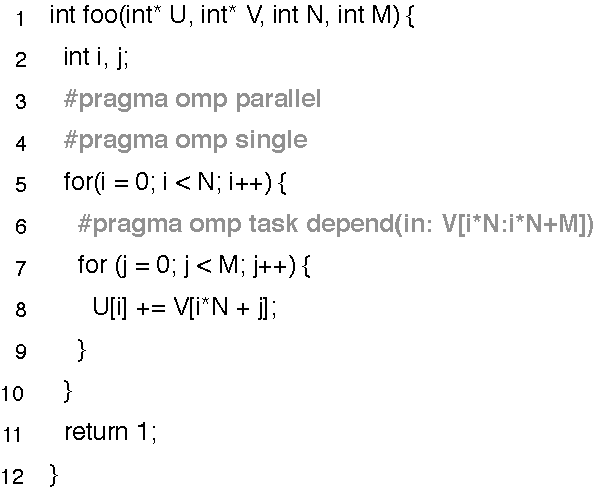
\includegraphics[width=0.95\columnwidth]{images/ex_Regions}
\caption{Write caption here.}
\label{fig:ex_Regions}
\end{center}
\end{figure}

\begin{Challenge}
\label{ch:cost}
Estimate the profitability of tasks at runtime.
\end{Challenge}

The creation of tasks involves a non-negligible runtime cost due to allocation and
scheduling of resources.
Ideally, this cost should be paid only for tasks that perform an amount of work
sufficiently large to pay for their management.
Being an interesting program property, on Rice's sense~\cite{Rice53}, the amount
of work performed by a task cannot be discovered statically.
As we show in Section~\ref{sub:profit}, we can try to approximate this quantity, using,
to this end, program symbols, which are replaced with actual values at runtime.
For instance, in Figure~\ref{fig:ex_Regions}, we know that the body of the
innermost loop is formed by five instructions.
Thus, we approximate the amount of work performed by a task with the
expression \textsf{5 * M}.
We use the runtime value of \textsf{M} to determine, during the execution of the
program, if we create a task, or not.
Such test is carried out by the guard at line 7 of the figure, which is part of
OpenMP's syntax.

\begin{Challenge}
\label{ch:cutoff}
Bound the creation of recursive tasks.
\end{Challenge}

We introduce Challenge~\ref{ch:cutoff} by quoting Duran {\em et al.}:
``{\em In task parallel languages, an important factor for achieving a good
performance is the use of a cut-off technique to reduce the number of tasks
created}"~\cite{Duran08}.
This observation is particularly true in the context of recursive, fine-grain,
tasks, as we analyze in Section~\ref{sub:rec}.
Figure~\ref{fig:ex_cutoff} provides such an example.
To place a limit on the number of tasks simultaneously in flight, we associate
the invocation of recursive functions annotated with task pragmas with a
counter -- \textsf{taskminer\_depth\_cutoff} in Figure~\ref{fig:ex_cutoff}.
The guard in line 7 ensures that we never exceed \textsf{DEPTH\_CUTOFF}, a
predetermined threshold.
This example, together with Figure~\ref{fig:ex_Regions}, lets us emphasize that
the code generation algorithms presented in this paper are
parameterized by constants such as \textsf{DEPTH\_CUTOFF}, or
\textsf{WORK\_CUTOFF} in Figure~\ref{fig:ex_Regions}.

\begin{figure}[t!]
\begin{center}
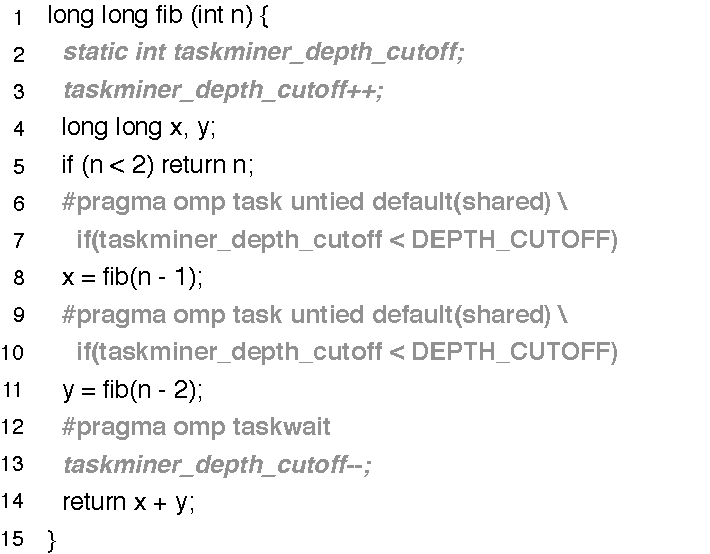
\includegraphics[width=0.95\columnwidth]{images/ex_cutoff}
\caption{Write caption here.}
\label{fig:ex_cutoff}
\end{center}
\end{figure}

\begin{Challenge}
\label{ch:privatize}
Identify private and shared variables.
\end{Challenge}

The two previous challenges are related to the performance of annotated
programs: if left unsolved, we shall have correct, albeit inefficient programs.
Challenges~\ref{ch:Regions}, and~\ref{ch:privatize}, in turn, are
related to correctness.
Challenge~\ref{ch:privatize} asks for the identification of variables that
must be replicated among threads.
This process of replication is called {\em privatization}.
As an example, variable \textsf{j} in Figure~\ref{fig:ex_privatize} must
be privatized.
In the absence of such action, that variable will be shared among all the
tasks created at line 5 of Figure~\ref{fig:ex_privatize}.
Because \textsf{j} is written within these tasks, race conditions would
ensue.
Section~\ref{sub:variance} explains how we separate private and
shared variables.

\begin{figure}[t!]
\begin{center}
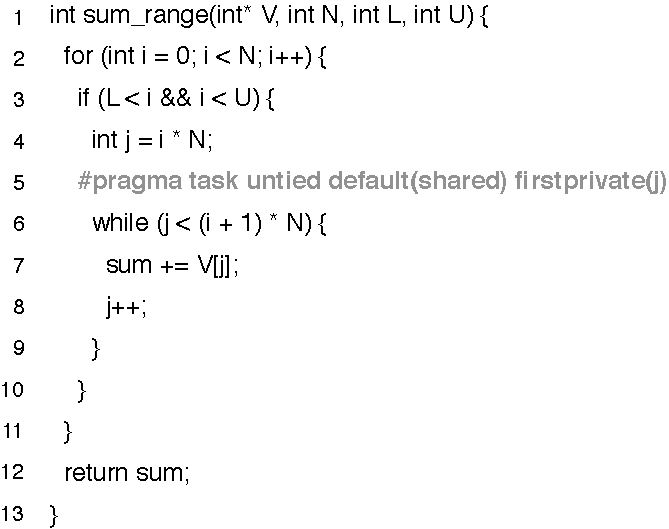
\includegraphics[width=1\columnwidth]{images/ex_privatize}
\caption{Write caption here.}
\label{fig:ex_privatize}
\end{center}
\end{figure}

% The ability to handle pointers through speculative parallelization.

% when applied to general-purpose integer-intensive applications that have complex control flow and excessive pointer accesses, traditional parallelization tech- niques become quite ineffective, as they need to conservatively ensure program correctness by synchronizing all potential dependences in the program

% For example in 473.astar if we ignore dependences that only occur in less than 20% of all iterations, we can parallelize loops that correspond to 96% of total execution.

\section{Solution}
\label{sec:sol}

\subsection{Mapping Program Regions to Tasks}
\label{sub:identification}

\subsection{Finding Symbolic Bounds of Arrays}
\label{sub:symb}

\subsection{Estimating the Profitability of Tasks}
\label{sub:profit}

\subsection{Limiting the Creation of Recursive Tasks}
\label{sub:rec}

\subsection{Separating Private from Shared Variables}
\label{sub:variance}

\subsection{Mapping IR onto Source Code}
\label{sub:ir}

\section{Evaluation}
\label{sec:eval}

We aimed to show that our tool exceeded in three main aspects that surround parallel programming. Thus our work evaluation stands on these 3 pillars:

% In section 4. “Evaluation", subsection “Performance"; you state the only reason why programmers will strive for parallelism would be to achieve higher performance (faster program execution). I do not fully agree, and I believe we discussed that point earlier. There may be cases where performance of a single big core would be good enough to meet some target schedule (either response time or frame rate, etc.) still you may want to explore parallel versions of the code running on a cluster of smaller cores or a combination of a slow CPU and GPU to achieve better power efficiency.

% I believe this paper could be made stronger by also investigating the impact of power efficiency as a component of the cost function - if one looks at the latest processor chips from Intel and AMD, I can (finally) see there is a trend to increase the number of cores for all platforms.

% In the past there has been not much opportunity to take advantage of parallelism on 2 core platforms (especially notebook designs used to limit the number of real cores), but with 6 or 8 core processors entering the main stream, we may take advantage of running more processors slower (lower voltage) or spreading out the workload over a larger die area. It is quite interesting to note that running one core hot will increase the leakage in that area of the die much more (exponentially with temperature), so distributing work over a larger die area results in reduced leakage - having said that, a similar effect can be achieved by migrating the workload from core to core.

\begin{itemize}

\item Practicality
\item Applicability
\item Performance

\end{itemize}

\textbf{\textit{Practicality}}. Programming in a parallel pattern is deemed difficult by programmers mainly because of the complexity of its data structures and algorithms. We show that our tool is simple and practical, for it does not involve changing the code and data structures in order to fit in a parallel pattern. The code is simply annotated by compiler directives.

\textbf{\textit{Applicability}}. 

\textbf{\textit{Performance}}. When it comes to parallel computing, it is undeniable that the main achievable goal should be performance. There's no reason why programmers would opt for parallelism other than the desire for faster programs. Therefore, we ought to show that the programs annotated with TaskMiner are faster than their serial counterparts. 

\section{Related Work}
\label{sec:rw}

% Talk about annotations vs libraries, e.g., Wool, Intel TBB. See: "A Comparison of some recent Task-based Parallel Programming Models"

\section{Conclusion}
\label{sec:conc}

\bibliography{references}

\end{document}
